%\textit{Conceptual Design Summary: 3-5 pages for this.  Begin the section by offering a high-level view of our final design highlighting the ways in which it meets the client requirements.}
 
\subsection{Analysis of Concept Selection}
%Here is where we will mention other designs that we considered.  We can go into them a little bit if needed, pointing out where they fell short of the final design, and where their strong points were.  Basically he says we “should focus on the ideas that directly led to your final conceptual design.” We can include pictures of actual prototypes we created as well as CAD models.  This is a brief walk-through of our design selection process to show that we considered and pursued multiple design options.  We want to basically back up our design choices with proofs and rational basis.

%\textbf{(Main point)}:  LOX compatibility was main design challenge, incorporated chemically inert PTFE to act as liner material on the inside of the tank to mitigate potential issues with varying designs.  PTFE became the driving component of each design due to different required dimensions.

The primary challenge of designing a composite fuel tank was making the tank compatible with LOX. Chemical incompatibility between LOX and the carbon fiber epoxy resin made this a potentially hazardous problem. In order to mitigate this issue, a chemically inert barrier was needed to line the inside of the tank and segregate these two materials. The material chosen for this purpose was polytetrafluoroethylene (PTFE). A detailed discussion of this design choice can be found in section 4.4.

PTFE is only readily available in a few basic geometries from vendors. The most convenient for use in a cylindrical tank are sheet and tube. Anticipating material and manufacturing lead times, the team chose to pursue two primary designs in parallel, one for each bulk material shape. Both were accomplished using a 3" inner diameter to save time and materials.   

\subsection{Sheet Design}

%\textbf{(Main Point)}: PTFE etched sheet was used/investigated, easier to obtain/manufacture, secured into cylindrical shape using Aluminum ‘bridge’.

	The sheet design has 1/32” thick PTFE liner. PTFE is known for having a very low coefficient of friction with nearly all other materials, making it very difficult to adhere to the other tank components. To overcome this, the liner material was chemically etched on the outside and then wrapped around a mandrel and secured into a cylindrical shape using a structural adhesive film known as Cytec Metlbond. A 1"-wide bridge made of 1/32" aluminum sheet was employed along the outside of the seam to seal it. (ref. Associated ring/cap designs). An inner layer of woven carbon fiber fabric, followed by a 1/4" layer of honeycomb patterned core material known as Nomex, and an outer layer of the same material as the inner layer were then wrapped over the liner, with adhesive film between each layer. Support structures were needed at the ends of the carbon fiber body to hold the layers in place during curing of the carbon fiber resin and adhesive, and during removal of the mandrel. This was accomplished via a thin cylinder that extended out of the rings and sandwiched between the liner and structural layers. These structures also provided a way to fasten end caps onto the tank and space for future module mating features. Henceforth, these structures will be referred to as mating rings (ref. dimensions/CAD whatever). End caps were necessary to close the tank and are enclosed within the rocket airframe. They feature holes for plumbing fixtures, and are each fastened to the mating rings with 12 axially aligned #3-48 stainless steel screws (ref. fasteners). 6061-T6 aircraft aluminum was chosen as the mating ring and end cap material. This design decision is detailed in section 4.1. The interface between the mating rings and end caps provided an escape path for the LOX, necessitating the use of a gasket. Again, PTFE was the chosen material here. The layup procedure for this design can be referenced in Appendix (#).
	
	An advantage of this design concept is the ease of its manufacture and reduced weight relative to the tube design. A PTFE oxygen permeability calculation found in Appendix (#) lead us to the conclusion that the liner would easily perform its function at a thickness as low as 0.02". 

\subsection{Tube Design}

%(Main Point):  The ‘ideal’ design, incorporates a tube of PTFE which provides a uniform liner surface with no seam in comparison to using a sheet, necessary to machine in house down to appropriate wall thickness (⅛”-1/16”)

	The second design deployed an unetched PTFE tube with a 1/8" wall thickness, using an altered ring/cap design to provide a shrink fit in order to seal the tank. Tubes were purchased at a 0.25” wall thickness, and then were manually turned down using a lathe to a $\frac{1}{8}$”  wall thickness to be incorporated into a layup.  (something along the lines of the difficulties or something regarding this issue, then referencing more detailed description below in subsystem highlights of manufacturing process developed to solve this issue) Coupled with the altered ring and endcap design (ref. Designs/dimensions) , the tube was inserted between the mating rings, with the end caps secured using a shrink fit to compress the cap onto the PTFE tube liner to provide a seal on the tank.  The material layers used in the sandwich layering were 2 layers of carbon fiber, one layer of 0.25” overexpanded nomex honeycomb, and one layer of 0.125” nonexpanded nomex honeycomb on the interior layer of the tank to account for the thicker ‘lapping portion’ of this mating ring design.  The layup procedure for this design can be referenced in Appendix \ref{appendix:Sub1}.
	There are two major advantages to this design. The first eliminates the extra seam caused by wrapping the PTFE sheet, which provides a more uniform interior liner. The second is that it does not require PTFE etching, or the addition of sealant along any interior edges or seams of the tank.
	
\subsection

    Although the sheet design was easier to manufacture, the shrink-fit tube design proved to be the superior design.  (ref flow chart & design scoring sheet if applicable).  As detailed below, testing yielded a positive result in all aspects of this tube tank design.  The sealing mechanism of the shrink fit was successful and provided minimal leakage when subjected to a hydrostatic burst test. (detail values here?)  Under compression loading at cryogenic temperatures the tube design withstood a load reaching 9500 lbs.  In contrast, the sheet design showed minimal success when subjected to hydrostatic pressure, and hence was abandoned.
    
    
    \begin{center}
    \centering
    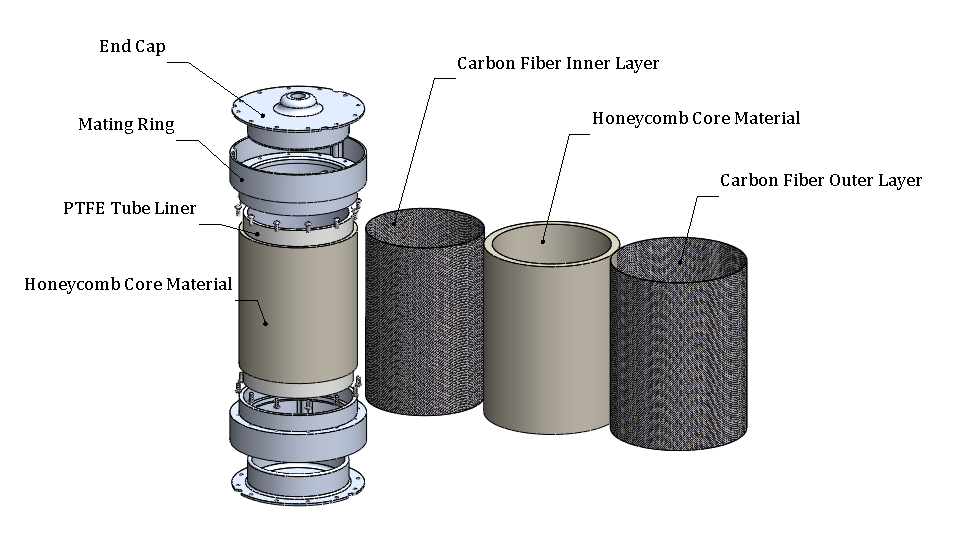
\includegraphics[width=\textwidth]{Cryo_Tank_explodedview_dimetric_crop.png}
    \captionof{figure}{Exploded View of Cryotank Layers}
    \label{fig:ExploadedView}
\end{center}
\newpage